\documentclass[../main.tex]{subfiles}
\begin{document}
\chapter{Arsitektur Mikroprosesor Intel 8086}

\section{Tujuan Pembelajaran}
Setelah mengikuti pertemuan ini, mahasiswa mampu:
\begin{itemize}
    \item Menggambarkan arsitektur internal Intel 8086 beserta karakteristik historisnya.
    \item Menjelaskan fungsi register-register utama (umum, indeks, pointer, segmen, IP, FLAGS).
    \item Menjelaskan segmentasi memori, pembentukan alamat fisik, dan batasan mode real.
    \item Menerapkan berbagai mode pengalamatan pada contoh instruksi sederhana.
    \item Menyusun struktur berkas ASM yang benar dengan direktif umum.
\end{itemize}

\section{Pendahuluan}
    Intel 8086, yang diperkenalkan pada tahun 1978, merupakan mikroprosesor 16-bit revolusioner yang menjadi fondasi arsitektur x86 yang masih digunakan hingga saat ini \cite{intel_8086_user_manual}. Mikroprosesor ini menandai era baru dalam komputasi personal dengan kemampuannya mengalamati hingga 1 MB memori melalui sistem segmentasi yang inovatif \cite{wiki_8086}. 

    Meskipun teknologi telah berkembang pesat selama lebih dari empat dekade, pemahaman mendalam tentang Intel 8086 tetap sangat penting karena beberapa alasan fundamental:

    \begin{itemize}
        \item \textbf{Kompatibilitas ke belakang}: Arsitektur modern x86/x64 tetap mempertahankan kompatibilitas dengan instruksi dan konsep dasar 8086
        \item \textbf{Pemrograman tingkat rendah}: Konsep register, segmentasi memori, dan mode pengalamatan yang diperkenalkan 8086 menjadi dasar pemahaman pemrograman assembly
        \item \textbf{Pemahaman sistem}: Memahami cara kerja mikroprosesor klasik membantu memahami evolusi dan kompleksitas sistem modern
        \item \textbf{Embedded systems}: Banyak sistem embedded masih menggunakan arsitektur serupa untuk aplikasi tertentu
    \end{itemize}

    Dalam bab ini, kita akan mempelajari secara mendalam arsitektur internal Intel 8086, sistem register yang kompleks, mekanisme segmentasi memori yang unik, dan berbagai mode pengalamatan yang memungkinkan fleksibilitas dalam pemrograman assembly.

\section{Arsitektur Dasar Intel 8086}

    \subsection{Sejarah dan Karakteristik Teknis}
        Intel 8086, yang diluncurkan pada Juni 1978, merupakan mikroprosesor 16-bit yang merevolusi industri komputer \cite{intel_8086_user_manual}. Mikroprosesor ini dikembangkan sebagai respons terhadap kebutuhan pasar akan prosesor yang lebih powerful dibandingkan pendahulunya, Intel 8080 dan 8085 \cite{brey1986mikroprosesor}.

        \begin{table}[H]
            \centering
            \caption{Spesifikasi Teknis Intel 8086}
            \begin{tabular}{|p{2.5cm}|p{2.8cm}|p{6cm}|}
\hline
\textbf{Aspek} & \textbf{Spesifikasi} & \textbf{Keterangan} \\
\hline
\textbf{Arsitektur} & 16-bit internal/eksternal & Data path dan register 16-bit \\
\hline
\textbf{Bus Alamat} & 20-bit & Pengalamatan hingga 1 MB (2$^{20}$ byte) \\
\hline
\textbf{Bus Data} & 16-bit & Transfer data 2 byte sekaligus \\
\hline
\textbf{Frekuensi Clock} & 5-10 MHz & Tergantung versi prosesor \\
\hline
\textbf{Transistor} & ~29,000 & Proses manufaktur 3-micron HMOS \\
\hline
\textbf{Konsumsi Daya} & ~2.5 watt & Relatif efisien untuk era tersebut \\
\hline
\textbf{Paket} & 40-pin DIP & Dual Inline Package standard \\
\hline
            \end{tabular}
            \label{tab:8086-specifications}
        \end{table}

        Intel 8086 menjadi dasar untuk seluruh keluarga prosesor x86 yang mengikuti, termasuk 80286, 80386, 80486, Pentium, dan bahkan prosesor modern Intel Core \cite{intel2019manual32}. Kompatibilitas ke belakang yang dipertahankan Intel memastikan bahwa program yang ditulis untuk 8086 masih dapat berjalan pada prosesor modern (dalam mode kompatibilitas).

    \subsection{Arsitektur internal mikroprosesor}
        Arsitektur internal Intel 8086 menggunakan desain \textit{pipelined} yang terdiri dari dua unit utama yang bekerja secara paralel untuk meningkatkan kinerja \cite{computer_organization_design}:

        \begin{figure}[H]
            \centering
            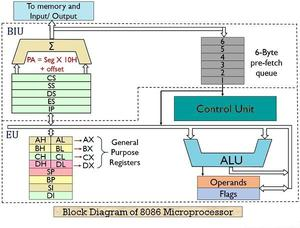
\includegraphics[width=0.7\textwidth]{../images/8086_architecture.jpg}
            \caption{Arsitektur Internal Intel 8086}
            \label{fig:8086-architecture}
        \end{figure}

        \begin{enumerate}
            \item \textbf{Bus Interface Unit (BIU)}
BIU bertanggung jawab untuk semua komunikasi dengan memori dan perangkat I/O eksternal. Unit ini memiliki beberapa komponen penting:

\begin{itemize}
    \item \textbf{Instruction Queue}: Buffer 6-byte yang menyimpan instruksi yang telah diambil dari memori
    \item \textbf{Segment Registers}: CS, DS, SS, ES untuk pengalamatan segmentasi
    \item \textbf{Instruction Pointer (IP)}: Menunjuk ke instruksi berikutnya yang akan dieksekusi
    \item \textbf{Address Adder}: Menghitung alamat fisik dari segment:offset
    \item \textbf{Bus Control Logic}: Mengatur sinyal kontrol bus (RD, WR, M/IO, dll.)
\end{itemize}

            \item \textbf{Execution Unit (EU)}
EU bertanggung jawab untuk eksekusi instruksi dan operasi aritmatika/logika:

\begin{itemize}
    \item \textbf{Arithmetic Logic Unit (ALU)}: Melakukan operasi aritmatika dan logika
    \item \textbf{General Purpose Registers}: AX, BX, CX, DX dan bagian 8-bitnya
    \item \textbf{Index and Pointer Registers}: SI, DI, SP, BP
    \item \textbf{Flag Register}: Menyimpan status hasil operasi
    \item \textbf{Control Unit}: Mengendalikan operasi EU dan komunikasi dengan BIU
\end{itemize}

        \begin{table}[H]
            \centering
            \caption{Komparasi Fungsi BIU dan EU}
            \begin{tabular}{|p{3.0cm}|p{5cm}|p{5cm}|}
\hline
\textbf{Aspek} & \textbf{Bus Interface Unit (BIU)} & \textbf{Execution Unit (EU)} \\
\hline
\textbf{Fungsi Utama} & Komunikasi dengan memori dan I/O & Eksekusi instruksi dan operasi \\
\hline
\textbf{Komponen} & Instruction Queue, Segment Registers, IP & ALU, General Registers, Flags \\
\hline
\textbf{Operasi} & Prefetch instruksi, hitung alamat fisik & Eksekusi instruksi, operasi aritmatika \\
\hline
\textbf{Kecepatan} & Berjalan paralel dengan EU & Bergantung pada kompleksitas instruksi \\
\hline
\textbf{Optimasi} & Prefetch queue (6 byte) & Pipeline dengan BIU \\
\hline
            \end{tabular}
            \label{tab:biu-eu-comparison}
        \end{table}

            \item \textbf{Mekanisme Prefetch Queue}
Salah satu inovasi penting 8086 adalah \textit{prefetch queue}. Ketika EU sedang mengeksekusi instruksi, BIU secara bersamaan mengambil instruksi berikutnya dari memori dan menyimpannya dalam queue 6-byte. Ini memungkinkan eksekusi yang lebih efisien karena instruksi sudah tersedia ketika EU membutuhkannya.

\begin{figure}[H]
    \centering
    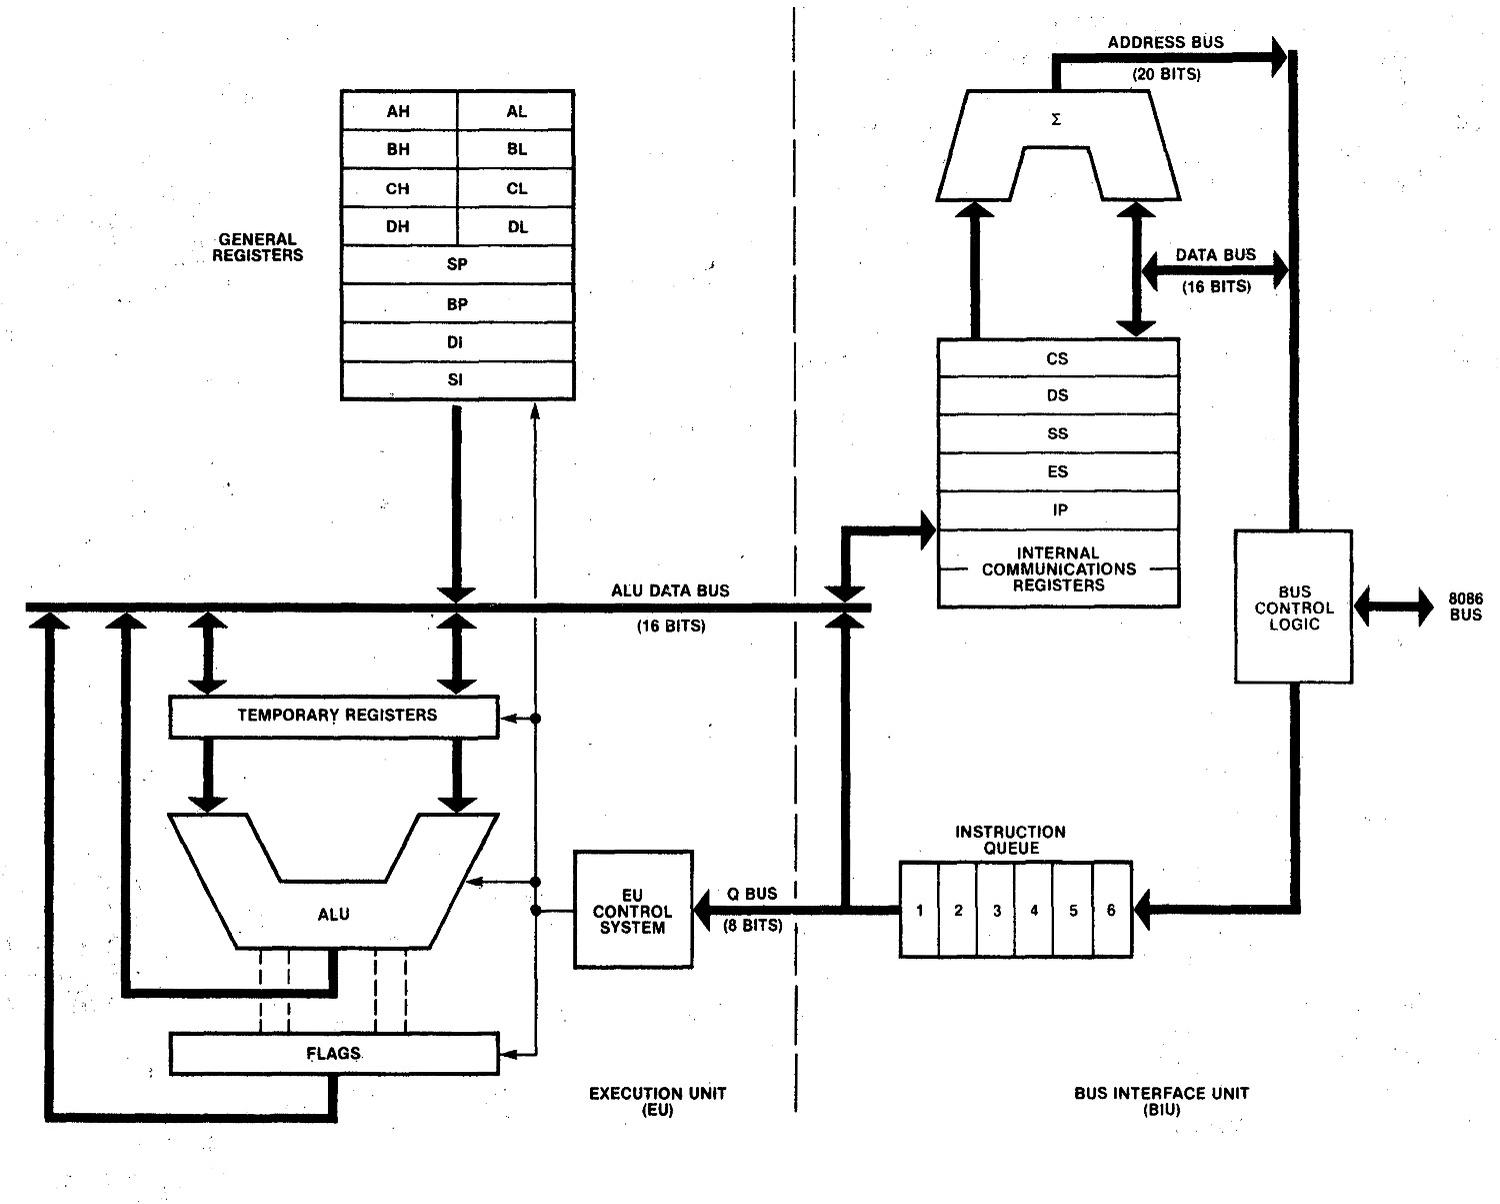
\includegraphics[width=0.6\textwidth]{../images/8086_prefetch_queue.jpg}
    \caption{Mekanisme Prefetch Queue Intel 8086}
    \label{fig:8086-prefetch-queue}
\end{figure}

            \item \textbf{Kerja Sama BIU dan EU}
\begin{enumerate}
    \item BIU mengambil instruksi dari memori dan menyimpannya dalam queue
    \item EU mengambil instruksi dari queue dan mengeksekusinya
    \item Jika EU memerlukan akses memori (operand), BIU menghentikan prefetch dan melayani permintaan EU
    \item Setelah akses memori selesai, BIU melanjutkan prefetch
\end{enumerate}
        \end{enumerate}

        \subsection{Bus sistem dan kontrol}
            Bus alamat 20-bit memungkinkan akses 1 MB (\(2^{20}\) byte). Bus data 16-bit memindahkan data per word. Sinyal kontrol (RD, WR, M/IO, INTA, dsb.) mengoordinasikan siklus baca/tulis memori dan I/O. Interupsi dapat memicu transfer kontrol ke \textit{interrupt vector table} di alamat rendah memori.

        \subsection{Mode operasi (real mode)}
            Pada 8086, hanya ada \textit{real mode}. Alamat fisik dihitung sebagai \(\text{segmen} \times 16 + \text{offset}\). Tidak ada proteksi memori atau \textit{paging}. Kode memiliki akses penuh ke seluruh ruang alamat 1 MB, yang menuntut disiplin pengaturan segmen.

    \section{Sistem Register Intel 8086}

        Intel 8086 memiliki sistem register yang kompleks dan terorganisir dengan baik. Register-register ini dapat dikelompokkan berdasarkan fungsinya, dan setiap register memiliki karakteristik dan penggunaan khusus yang penting untuk dipahami dalam pemrograman assembly.

        \begin{table}[H]
            \centering
            \caption{Klasifikasi Register Intel 8086}
            \begin{tabular}{|p{2.8cm}|p{3.2cm}|p{6.2cm}|}
\hline
\textbf{Kategori} & \textbf{Register} & \textbf{Deskripsi} \\
\hline
\textbf{General Purpose} & AX, BX, CX, DX & Register 16-bit yang dapat diakses sebagai 8-bit (AH/AL, BH/BL, CH/CL, DH/DL) \\
\hline
\textbf{Index Registers} & SI, DI & Source Index dan Destination Index untuk operasi string \\
\hline
\textbf{Pointer Registers} & SP, BP & Stack Pointer dan Base Pointer untuk manajemen stack \\
\hline
\textbf{Segment Registers} & CS, DS, SS, ES & Code, Data, Stack, dan Extra Segment untuk segmentasi memori \\
\hline
\textbf{Control Registers} & IP, FLAGS & Instruction Pointer dan Flag Register untuk kontrol eksekusi \\
\hline
            \end{tabular}
            \label{tab:register-classification}
        \end{table}

        \begin{figure}[H]
            \centering
            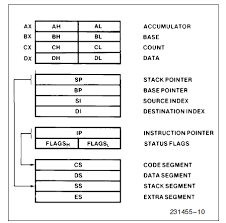
\includegraphics[width=0.7\textwidth]{../images/8086_registers.png}
            \caption{Register-Register Intel 8086}
            \label{fig:8086-registers}
        \end{figure}

        \subsection{Register umum (AX, BX, CX, DX)}
            Register umum adalah jantung dari operasi aritmatika dan manipulasi data dalam Intel 8086. Keempat register ini memiliki karakteristik unik dan penggunaan khusus yang telah menjadi konvensi dalam pemrograman assembly.

            \begin{centeredlongtable}{|L{1.2cm}|L{1.6cm}|L{2.0cm}|L{3.6cm}|}
                \caption{Detail Register Umum Intel 8086}\\
                \hline
                \textbf{Register} & \textbf{Nama Lengkap} & \textbf{Bagian 8-bit} & \textbf{Fungsi Utama dan Penggunaan Khusus} \\
                \hline
                \endfirsthead
                
                \multicolumn{4}{c}%
                {{\bfseries \tablename\ \thetable{} -- lanjutan dari halaman sebelumnya}} \\
                \hline
                \textbf{Register} & \textbf{Nama Lengkap} & \textbf{Bagian 8-bit} & \textbf{Fungsi Utama dan Penggunaan Khusus} \\
                \hline
                \endhead
                
                \hline \multicolumn{4}{|r|}{{Lanjutan di halaman berikutnya}} \\ \hline
                \endfoot
                
                \hline
                \endlastfoot
                
                \textbf{AX} & Accumulator & AH (High), AL (Low) & \begin{itemize}
                \item Operasi aritmatika utama (ADD, SUB, MUL, DIV)
                \item Operasi I/O (IN, OUT)
                \item Konversi data dan operasi khusus
                \item Return value dari fungsi
                \end{itemize} \\
                \hline
                \textbf{BX} & Base Register & BH (High), BL (Low) & \begin{itemize}
                \item Base address untuk pengalamatan memori
                \item Array indexing dengan displacement
                \item Pointer ke struktur data
                \item Offset dalam segmentasi memori
                \end{itemize} \\
                \hline
                \textbf{CX} & Count Register & CH (High), CL (Low) & \begin{itemize}
                \item Counter untuk instruksi LOOP
                \item Counter untuk instruksi REP (string operations)
                \item Shift/rotate count untuk SHL, SHR, ROL, ROR
                \item Loop control dalam algoritma
                \end{itemize} \\
                \hline
                \textbf{DX} & Data Register & DH (High), DL (Low) & \begin{itemize}
                \item Extended accumulator untuk operasi 32-bit
                \item Port I/O untuk operasi IN/OUT dengan port > 255
                \item Dividend high untuk operasi DIV
                \item Multiplier high untuk operasi MUL
                \end{itemize} \\
                \label{tab:general-registers-detail}
            \end{centeredlongtable}

            \textbf{Karakteristik Penting Register Umum:}

            \textbf{1. Akses Dual (16-bit dan 8-bit)}
Setiap register umum dapat diakses sebagai register 16-bit penuh atau sebagai dua register 8-bit terpisah. Contoh:
\begin{lstlisting}[language={[x86masm]Assembler}, caption=Akses Dual Register 8086, label=lst:dual-access]
mov ax, 1234h    ; Mengisi AX dengan 1234h
mov ah, 12h      ; Mengisi AH dengan 12h (high byte)
mov al, 34h      ; Mengisi AL dengan 34h (low byte)
\end{lstlisting}

            \textbf{2. Konvensi Penggunaan}
Meskipun secara teknis semua register umum dapat digunakan untuk operasi apapun, konvensi pemrograman assembly telah menetapkan penggunaan khusus untuk setiap register:

\begin{itemize}
    \item \textbf{AX}: Selalu digunakan sebagai akumulator utama untuk operasi aritmatika
    \item \textbf{BX}: Digunakan sebagai base register untuk pengalamatan memori
    \item \textbf{CX}: Digunakan sebagai counter untuk loop dan operasi string
    \item \textbf{DX}: Digunakan untuk operasi extended precision dan I/O
\end{itemize}

            \textbf{3. Penggunaan dalam Instruksi Khusus}
Beberapa instruksi memiliki ketergantungan khusus pada register tertentu:

\begin{table}[H]
    \centering
    \caption{Instruksi dengan Ketergantungan Register}
    \begin{tabular}{|p{2.2cm}|p{3.2cm}|p{6.2cm}|}
        \hline
        \textbf{Instruksi} & \textbf{Register yang Digunakan} & \textbf{Keterangan} \\
        \hline
        \texttt{MUL} & AX, DX & AX = multiplicand, DX:AX = hasil \\
        \hline
        \texttt{DIV} & AX, DX & AX = dividend, DX = remainder \\
        \hline
        \texttt{LOOP} & CX & CX = counter, decrement otomatis \\
        \hline
        \texttt{REP} & CX & CX = repeat count untuk string ops \\
        \hline
        \texttt{IN/OUT} & AL/AX & AL untuk port < 256, AX untuk port > 255 \\
        \hline
        \texttt{SHL/SHR} & CL & CL = shift count \\
        \hline
    \end{tabular}
    \label{tab:instruction-register-dependency}
\end{table}

        \subsection{Register Indeks dan Pointer}\label{subsec:arsitektur-indeks-pointer}
            Register indeks dan pointer memainkan peran penting dalam pengalamatan memori dan manajemen stack. Mereka memungkinkan akses yang fleksibel ke data dalam memori dan mendukung operasi string yang efisien.

            \subsubsection{Register indeks (SI, DI)}
Register indeks SI (Source Index) dan DI (Destination Index) adalah register 16-bit yang dirancang khusus untuk operasi string dan pengalamatan array. Mereka bekerja dalam kombinasi dengan register segmen untuk membentuk alamat memori yang efektif.

\begin{table}[H]
    \centering
    \caption{Detail Register Indeks SI dan DI}
    \begin{tabular}{|p{1.8cm}|p{3.2cm}|p{7.2cm}|}
        \hline
        \textbf{Register} & \textbf{Nama Lengkap} & \textbf{Fungsi dan Penggunaan} \\
        \hline
        \textbf{SI} & Source Index & \begin{itemize}
        \item Menunjuk ke elemen sumber dalam operasi string
        \item Default segment: DS (Data Segment)
        \item Digunakan dengan instruksi: MOVS, CMPS, LODS
        \item Increment/decrement otomatis setelah operasi string
        \item Dapat digunakan untuk array indexing
        \end{itemize} \\
        \hline
        \textbf{DI} & Destination Index & \begin{itemize}
        \item Menunjuk ke elemen tujuan dalam operasi string
        \item Default segment: ES (Extra Segment)
        \item Digunakan dengan instruksi: MOVS, CMPS, STOS
        \item Increment/decrement otomatis setelah operasi string
        \item Dapat digunakan untuk array indexing
        \end{itemize} \\
        \hline
    \end{tabular}
    \label{tab:index-registers-detail}
\end{table}

\textbf{Penggunaan dalam Operasi String:}
\begin{lstlisting}[language={[x86masm]Assembler}, caption=Operasi String dengan SI dan DI, label=lst:string-operations]
; Contoh operasi string dengan SI dan DI
mov si, offset source_string    ; SI menunjuk ke string sumber
mov di, offset dest_string      ; DI menunjuk ke string tujuan
mov cx, 10                      ; CX = panjang string
rep movsb                       ; Copy 10 bytes dari DS:SI ke ES:DI
\end{lstlisting}

\textbf{Penggunaan dalam Array Indexing:}
\begin{lstlisting}[language={[x86masm]Assembler}, caption=Akses Array dengan SI, label=lst:array-indexing]
; Contoh akses array dengan SI
mov si, 0                       ; SI = index awal
mov ax, array[si]               ; AX = array[0]
add si, 2                       ; SI = index berikutnya (word array)
mov bx, array[si]               ; BX = array[1]
\end{lstlisting}

            \subsubsection{Register pointer (SP, BP)}
Register pointer SP (Stack Pointer) dan BP (Base Pointer) adalah register 16-bit yang mengelola stack dan frame pointer untuk prosedur. Mereka bekerja dengan register segmen SS (Stack Segment).

\begin{table}[H]
    \centering
    \caption{Detail Register Pointer SP dan BP}
    \begin{tabular}{|p{1.8cm}|p{3.2cm}|p{7.2cm}|}
        \hline
        \textbf{Register} & \textbf{Nama Lengkap} & \textbf{Fungsi dan Penggunaan} \\
        \hline
        \textbf{SP} & Stack Pointer & \begin{itemize}
        \item Menunjuk ke puncak stack (top of stack)
        \item Default segment: SS (Stack Segment)
        \item Diubah otomatis oleh PUSH, POP, CALL, RET
        \item Harus dijaga keseimbangan stack
        \item Tidak boleh diubah manual kecuali hati-hati
        \end{itemize} \\
        \hline
        \textbf{BP} & Base Pointer & \begin{itemize}
        \item Base pointer untuk akses parameter dan variabel lokal
        \item Default segment: SS (Stack Segment)
        \item Digunakan untuk membuat stack frame
        \item Memungkinkan akses parameter dengan offset tetap
        \item Lebih stabil daripada SP untuk akses stack
        \end{itemize} \\
        \hline
    \end{tabular}
    \label{tab:pointer-registers-detail}
\end{table}

\textbf{Stack Frame dengan BP:}
\begin{lstlisting}[language={[x86masm]Assembler}, caption=Stack Frame dengan Base Pointer, label=lst:stack-frame]
; Contoh penggunaan BP untuk stack frame
push bp                         ; Simpan BP lama
mov bp, sp                      ; BP = SP (base of frame)
sub sp, 4                       ; Alokasi 4 byte untuk variabel lokal

; Akses parameter (di atas BP)
mov ax, [bp+6]                  ; Parameter pertama
mov bx, [bp+4]                  ; Parameter kedua

; Akses variabel lokal (di bawah BP)
mov [bp-2], ax                  ; Variabel lokal pertama
mov [bp-4], bx                  ; Variabel lokal kedua

mov sp, bp                      ; Restore SP
pop bp                          ; Restore BP lama
ret                             ; Return
\end{lstlisting}

% \begin{figure}[h]
% \centering
% 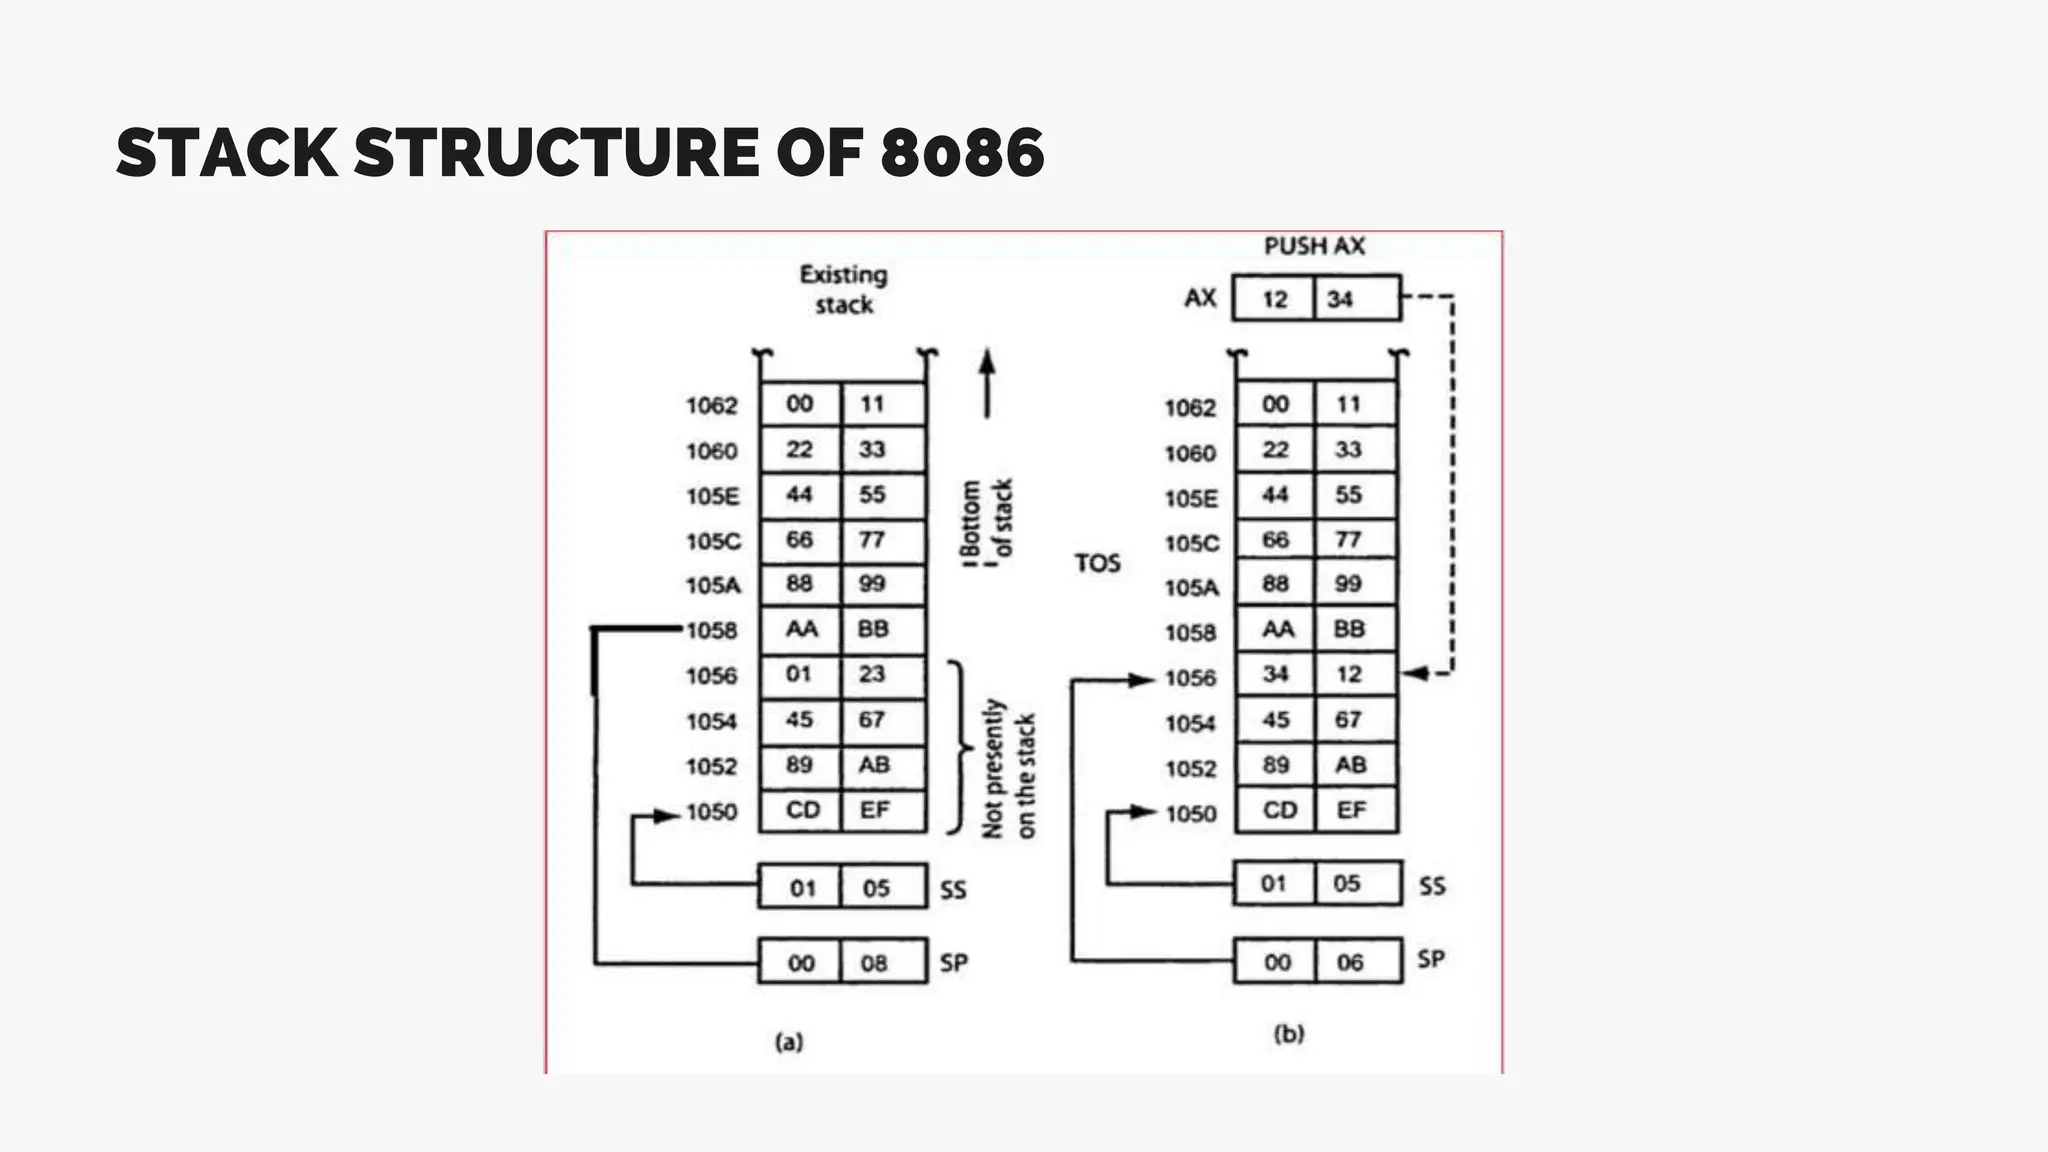
\includegraphics[width=0.7\textwidth]{../images/8086_stack_frame.jpg}
% \caption{Struktur Stack Frame Intel 8086}
% \label{fig:8086-stack-frame}
% \end{figure}

\textbf{Perbedaan Penting antara SP dan BP:}
\begin{itemize}
    \item \textbf{SP}: Selalu menunjuk ke puncak stack yang aktif, berubah dengan setiap operasi stack
    \item \textbf{BP}: Menunjuk ke base frame yang stabil, tidak berubah selama prosedur aktif
    \item \textbf{Akses}: SP untuk operasi stack (PUSH/POP), BP untuk akses parameter/lokal
    \item \textbf{Stabilitas}: BP lebih stabil untuk akses berulang ke data stack
\end{itemize}

        \subsection{Register Segmen dan Kontrol}\label{subsec:arsitektur-segmen-kontrol}
            Register segmen dan kontrol adalah komponen fundamental dalam arsitektur Intel 8086 yang memungkinkan sistem segmentasi memori yang unik. Mereka bekerja bersama untuk membentuk alamat fisik dan mengatur eksekusi program.

            \subsubsection{Register segmen (CS, DS, SS, ES)}
Register segmen adalah register 16-bit yang menentukan segmen memori yang sedang aktif. Setiap register segmen memiliki fungsi khusus dan bekerja dengan register offset untuk membentuk alamat fisik 20-bit.

\begin{centeredlongtable}{|L{1.0cm}|L{1.8cm}|L{2.4cm}|L{3.8cm}|}
    \caption{Detail Register Segmen Intel 8086}\\
    \hline
    \textbf{Register} & \textbf{Nama Lengkap} & \textbf{Default Offset} & \textbf{Fungsi dan Penggunaan} \\
    \hline
    \endfirsthead
    
    \multicolumn{4}{c}%
    {{\bfseries \tablename\ \thetable{} -- lanjutan dari halaman sebelumnya}} \\
    \hline
    \textbf{Register} & \textbf{Nama Lengkap} & \textbf{Default Offset} & \textbf{Fungsi dan Penggunaan} \\
    \hline
    \endhead
    
    \hline \multicolumn{4}{|r|}{{Lanjutan di halaman berikutnya}} \\ \hline
    \endfoot
    
    \hline
    \endlastfoot
    
    \textbf{CS} & Code Segment & IP (Instruction Pointer) & \begin{itemize}
    \item Menentukan segmen untuk eksekusi instruksi
    \item Tidak dapat diubah langsung (hanya melalui CALL, JMP, INT)
    \item Menentukan lokasi kode program dalam memori
    \item Bersama IP membentuk alamat instruksi berikutnya
    \end{itemize} \\
    \hline
    \textbf{DS} & Data Segment & BX, SI, DI, displacement & \begin{itemize}
    \item Menentukan segmen untuk akses data umum
    \item Default untuk sebagian besar operasi memori
    \item Dapat diubah dengan instruksi MOV
    \item Digunakan untuk variabel global dan array
    \end{itemize} \\
    \hline
    \textbf{SS} & Stack Segment & SP, BP & \begin{itemize}
    \item Menentukan segmen untuk operasi stack
    \item Default untuk PUSH, POP, CALL, RET
    \item Digunakan untuk parameter dan variabel lokal
    \item Harus dijaga konsistensi dengan SP/BP
    \end{itemize} \\
    \hline
    \textbf{ES} & Extra Segment & DI (untuk string ops) & \begin{itemize}
    \item Segmen tambahan untuk operasi khusus
    \item Default tujuan untuk instruksi string
    \item Dapat digunakan untuk akses data tambahan
    \item Fleksibel untuk berbagai keperluan
    \end{itemize} \\
    \label{tab:segment-registers-detail}
\end{centeredlongtable}

\textbf{Konsep Segmentasi Memori:}
Segmentasi memori adalah fitur unik Intel 8086 yang memecah ruang alamat 1 MB menjadi segmen-segmen logis yang dapat diakses secara independen. Setiap segmen memiliki ukuran maksimal 64 KB (2$^{16}$ byte).

\textbf{Perhitungan Alamat Fisik:}
\begin{center}
    \textbf{Alamat Fisik = (Segment Register $\times$ 16) + Offset}
\end{center}

\textbf{Contoh Perhitungan:}
\begin{itemize}
    \item CS = 2000h, IP = 0100h $\rightarrow$ Alamat Fisik = (2000h $\times$ 16) + 0100h = 20000h + 0100h = 20100h
    \item DS = 3000h, BX = 0040h $\rightarrow$ Alamat Fisik = (3000h $\times$ 16) + 0040h = 30000h + 0040h = 30040h
\end{itemize}

\textbf{Segment Overlap:}
Karena perhitungan alamat fisik menggunakan perkalian dengan 16, segmen dapat saling tumpang tindih:
\begin{itemize}
    \item Segmen 1000h:0000h = Alamat Fisik 10000h
    \item Segmen 1001h:0000h = Alamat Fisik 10010h
    \item Segmen 1000h:0010h = Alamat Fisik 10010h (sama dengan segmen kedua)
\end{itemize}

            \subsubsection{Register flag (FLAGS)}
Register FLAGS adalah register 16-bit yang menyimpan status hasil operasi dan mengendalikan perilaku prosesor. Setiap bit memiliki fungsi khusus yang penting untuk pemrograman assembly.

\begin{figure}[H]
    \centering
    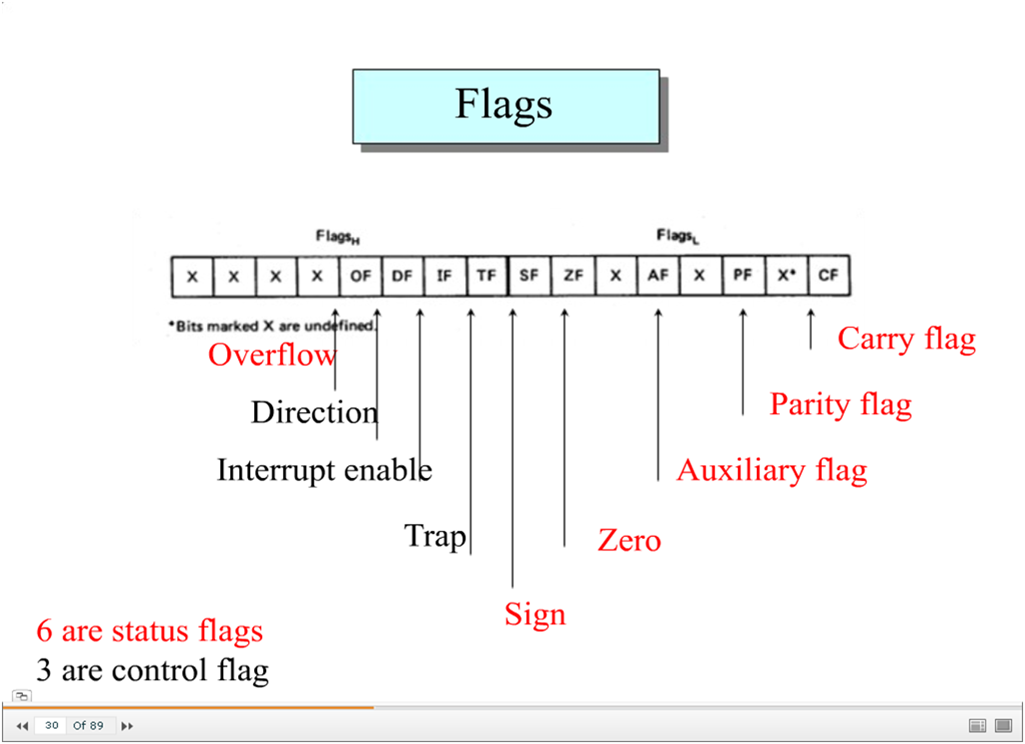
\includegraphics[width=0.7\textwidth]{../images/8086_flags_register.png}
    \caption{Register FLAGS Intel 8086}
    \label{fig:8086-flags-register}
\end{figure}

\begin{centeredlongtable}{|L{1.4cm}|L{2.2cm}|L{1.8cm}|L{5.8cm}|}
    \caption{Detail Register FLAGS Intel 8086}\\
    \hline
    \textbf{Bit} & \textbf{Nama Flag} & \textbf{Singkatan} & \textbf{Fungsi dan Kondisi Set} \\
    \hline
    \endfirsthead
    
    \multicolumn{4}{c}%
    {{\bfseries \tablename\ \thetable{} -- lanjutan dari halaman sebelumnya}} \\
    \hline
    \textbf{Bit} & \textbf{Nama Flag} & \textbf{Singkatan} & \textbf{Fungsi dan Kondisi Set} \\
    \hline
    \endhead
    
    \hline \multicolumn{4}{|r|}{{Lanjutan di halaman berikutnya}} \\ \hline
    \endfoot
    
    \hline
    \endlastfoot
    
    \textbf{0} & Carry Flag & CF & Carry dari operasi aritmatika (set jika ada carry out dari MSB) \\
    \hline
    \textbf{1} & Reserved & - & Dicadangkan untuk penggunaan masa depan \\
    \hline
    \textbf{2} & Parity Flag & PF & Parity genap dari hasil operasi (set jika jumlah bit 1 genap) \\
    \hline
    \textbf{3} & Reserved & - & Dicadangkan untuk penggunaan masa depan \\
    \hline
    \textbf{4} & Auxiliary Carry & AF & Carry dari nibble rendah ke nibble tinggi (BCD arithmetic) \\
    \hline
    \textbf{5} & Reserved & - & Dicadangkan untuk penggunaan masa depan \\
    \hline
    \textbf{6} & Zero Flag & ZF & Set jika hasil operasi adalah nol \\
    \hline
    \textbf{7} & Sign Flag & SF & Set jika hasil operasi negatif (MSB = 1) \\
    \hline
    \textbf{8} & Trap Flag & TF & Set untuk single-step debugging \\
    \hline
    \textbf{9} & Interrupt Flag & IF & Set untuk mengaktifkan interupsi maskable \\
    \hline
    \textbf{10} & Direction Flag & DF & Set untuk decrement dalam operasi string \\
    \hline
    \textbf{11} & Overflow Flag & OF & Set jika overflow dalam operasi aritmatika bertanda \\
    \hline
    \textbf{12-15} & Reserved & - & Dicadangkan untuk penggunaan masa depan \\
    \label{tab:flags-register-detail}
\end{centeredlongtable}

\textbf{Flag Penting untuk Pemrograman:}

\textbf{1. Status Flags (CF, PF, AF, ZF, SF, OF):}
\begin{itemize}
    \item \textbf{CF (Carry Flag)}: Penting untuk aritmatika tak bertanda dan operasi shift/rotate
    \item \textbf{ZF (Zero Flag)}: Digunakan untuk conditional jumps (JE, JNE, JZ, JNZ)
    \item \textbf{SF (Sign Flag)}: Digunakan untuk conditional jumps berdasarkan tanda (JL, JG, JLE, JGE)
    \item \textbf{OF (Overflow Flag)}: Penting untuk aritmatika bertanda dan deteksi overflow
\end{itemize}

\textbf{2. Control Flags (TF, IF, DF):}
\begin{itemize}
    \item \textbf{TF (Trap Flag)}: Mengaktifkan single-step mode untuk debugging
    \item \textbf{IF (Interrupt Flag)}: Mengontrol apakah interupsi maskable dapat terjadi
    \item \textbf{DF (Direction Flag)}: Mengontrol arah operasi string (increment/decrement)
\end{itemize}

\textbf{Contoh Penggunaan Flag:}
\begin{lstlisting}[language={[x86masm]Assembler}, caption=Penggunaan Flag untuk Conditional Jump, label={lst:flag-usage-ch02}]
; Contoh penggunaan flag untuk conditional jump
cmp ax, bx          ; Compare AX dengan BX
je equal            ; Jump jika equal (ZF = 1)
jl less_than        ; Jump jika less (SF != OF)
jg greater_than     ; Jump jika greater (ZF = 0 dan SF = OF)

; Contoh penggunaan flag untuk aritmatika
add ax, bx          ; Add BX ke AX
jc carry_occurred   ; Jump jika carry (CF = 1)
jo overflow_occurred ; Jump jika overflow (OF = 1)
\end{lstlisting}

\subsubsection{Register instruksi (IP)}
    Instruction Pointer (IP) adalah register 16-bit yang menyimpan offset instruksi berikutnya yang akan dieksekusi dalam segmen kode. IP bekerja bersama dengan CS untuk membentuk alamat fisik instruksi.

    \textbf{Karakteristik IP:}
    \begin{itemize}
        \item \textbf{Ukuran}: 16-bit (0-65535)
        \item \textbf{Segment}: Selalu menggunakan CS sebagai segment register
        \item \textbf{Update}: Diubah otomatis setelah setiap instruksi dieksekusi
        \item \textbf{Akses}: Tidak dapat diakses langsung, hanya melalui CALL, JMP, RET
    \end{itemize}

    \textbf{Operasi yang Mengubah IP:}
    \begin{table}[H]
        \centering
        \caption{Instruksi yang Mengubah IP}
        \begin{tabular}{|p{2.8cm}|p{3.8cm}|p{7cm}|}
            \hline
            \textbf{Instruksi} & \textbf{Jenis Operasi} & \textbf{Efek pada IP} \\
            \hline
            \texttt{JMP} & Unconditional Jump & IP = target address \\
            \hline
            \texttt{CALL} & Procedure Call & IP = target, return address pushed to stack \\
            \hline
            \texttt{RET} & Return from Procedure & IP = popped from stack \\
            \hline
            \texttt{INT} & Software Interrupt & IP = interrupt vector, flags pushed \\
            \hline
            \texttt{IRET} & Return from Interrupt & IP = popped from stack \\
            \hline
            \texttt{LOOP} & Conditional Loop & IP = target if CX $\neq$ 0 \\
            \hline
            \texttt{Jcc} & Conditional Jump & IP = target if condition true \\
            \hline
        \end{tabular}
        \label{tab:ip-modifying-instructions}
    \end{table}

    \section{Segmentasi Memori Intel 8086}
        Segmentasi memori adalah salah satu fitur paling inovatif dari Intel 8086 yang memungkinkan pengalamatan memori yang fleksibel dan efisien. Sistem ini memecah ruang alamat fisik 1 MB menjadi segmen-segmen logis yang dapat diakses secara independen.

        \begin{figure}[H]
            \centering
            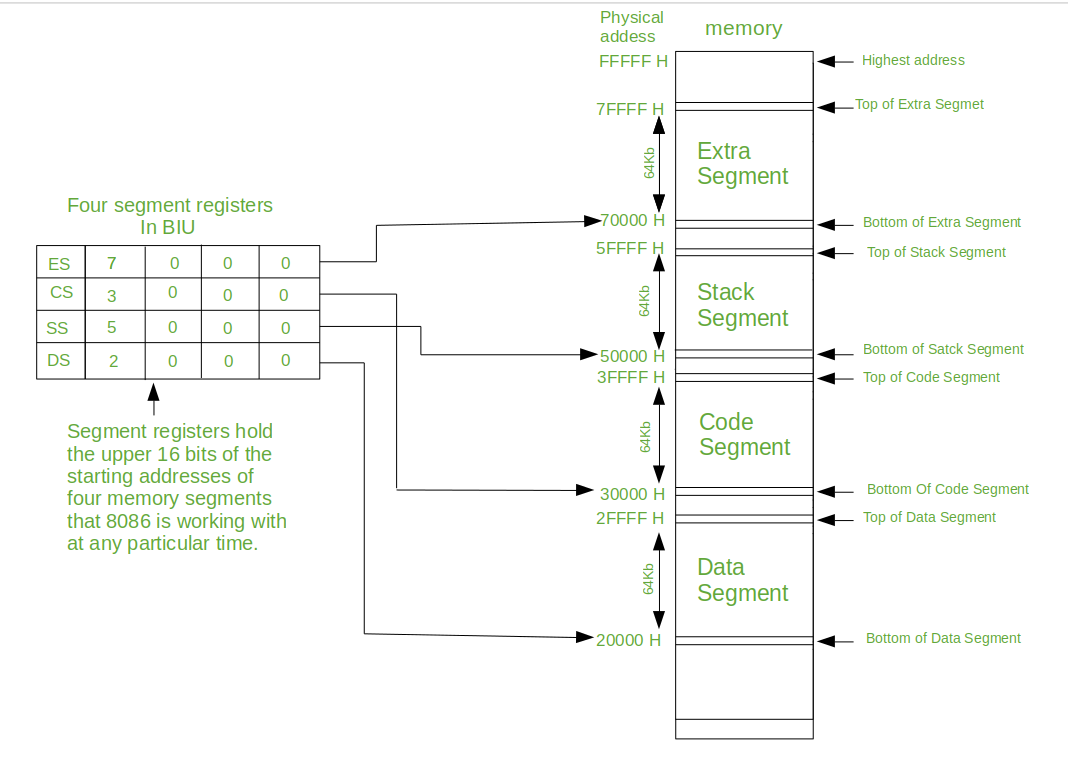
\includegraphics[width=0.7\textwidth]{../images/8086_memory_segmentation.png}
            \caption{Segmentasi Memori Intel 8086}
            \label{fig:8086-memory-segmentation}
        \end{figure}

        \subsection{Konsep Dasar Segmentasi}
            Segmentasi memori bekerja dengan membagi ruang alamat fisik menjadi blok-blok logis yang disebut segmen. Setiap segmen memiliki karakteristik khusus dan digunakan untuk tujuan tertentu dalam program.

            \begin{table}[H]
\centering
\caption{Karakteristik Segmentasi Memori Intel 8086}
\begin{tabular}{|p{3.2cm}|p{3.8cm}|p{7cm}|}
    \hline
    \textbf{Aspek} & \textbf{Nilai} & \textbf{Keterangan} \\
    \hline
    \textbf{Alamat Fisik} & 20-bit & Memungkinkan akses hingga 1 MB memori \\
    \hline
    \textbf{Alamat Logis} & 16-bit segment + 16-bit offset & Total 32-bit untuk alamat logis \\
    \hline
    \textbf{Ukuran Segmen} & 64 KB maksimal & Batasan offset 16-bit \\
    \hline
    \textbf{Segment Overlap} & 16-byte boundary & Setiap segmen dimulai pada kelipatan 16 \\
    \hline
    \textbf{Segment Registers} & 4 register aktif & CS, DS, SS, ES \\
    \hline
    \textbf{Memory Protection} & Tidak ada & Real mode tidak memiliki proteksi \\
    \hline
\end{tabular}
\label{tab:memory-segmentation-characteristics}
            \end{table}

        \subsection{Keuntungan dan Keterbatasan Segmentasi}
            \textbf{Keuntungan Segmentasi:}
            \begin{enumerate}
\item \textbf{Organisasi Program}: Memisahkan kode, data, dan stack secara logis
\item \textbf{Relokasi}: Program dapat dijalankan di lokasi memori yang berbeda
\item \textbf{Proteksi Dasar}: Meskipun terbatas, memberikan isolasi antar segmen
\item \textbf{Efisiensi Memori}: Memungkinkan penggunaan memori yang lebih efisien
            \end{enumerate}

            \textbf{Keterbatasan Segmentasi:}
            \begin{enumerate}
\item \textbf{Tidak Ada Proteksi Nyata}: Program dapat mengakses segmen lain
\item \textbf{Kompleksitas}: Menambah kompleksitas dalam pemrograman
\item \textbf{Overhead}: Perhitungan alamat fisik memerlukan operasi tambahan
            \end{enumerate}

        \subsection{Perhitungan Alamat Fisik}
            Perhitungan alamat fisik adalah proses mengkonversi alamat logis (segment:offset) menjadi alamat fisik 20-bit yang dapat digunakan untuk mengakses memori.

            \textbf{Rumus Perhitungan:}
            \begin{center}
\textbf{Alamat Fisik = (Segment Register $\times$ 16) + Offset}
            \end{center}

            \begin{table}[H]
\centering
\caption{Contoh Perhitungan Alamat Fisik}
\begin{tabular}{|p{2.8cm}|p{2.8cm}|p{2.8cm}|p{5.2cm}|}
    \hline
    \textbf{Segment} & \textbf{Offset} & \textbf{Perhitungan} & \textbf{Alamat Fisik} \\
    \hline
    2000h & 0100h & (2000h $\times$ 16) + 0100h & 20100h \\
    \hline
    3000h & 0040h & (3000h $\times$ 16) + 0040h & 30040h \\
    \hline
    1000h & 0010h & (1000h $\times$ 16) + 0010h & 10010h \\
    \hline
    1001h & 0000h & (1001h $\times$ 16) + 0000h & 10010h \\
    \hline
\end{tabular}
\label{tab:physical-address-calculation}
            \end{table}

            \textbf{Segment Overlap:}
            Dari tabel di atas, terlihat bahwa segmen 1000h:0010h dan 1001h:0000h menghasilkan alamat fisik yang sama (10010h). Ini menunjukkan bahwa segmen dapat saling tumpang tindih.

        \subsection{Batasan Mode Real}
            Mode real adalah satu-satunya mode operasi yang tersedia pada Intel 8086. Mode ini memiliki beberapa batasan penting:

            \begin{table}[H]
\centering
\caption{Batasan Mode Real Intel 8086}
\begin{tabular}{|p{3.2cm}|p{3.8cm}|p{7cm}|}
    \hline
    \textbf{Batasan} & \textbf{Nilai} & \textbf{Dampak pada Pemrograman} \\
    \hline
    \textbf{Ukuran Segmen} & 64 KB maksimal & Program besar harus dibagi menjadi beberapa segmen \\
    \hline
    \textbf{Proteksi Memori} & Tidak ada & Program dapat mengakses seluruh ruang memori \\
    \hline
    \textbf{Address Space} & 1 MB total & Terbatas untuk aplikasi modern \\
    \hline
    \textbf{Segment Overlap} & 16-byte boundary & Dapat menyebabkan konflik alamat \\
    \hline
\end{tabular}
\label{tab:real-mode-limitations}
            \end{table}

    \section{Mode Pengalamatan}

        Intel 8086 mendukung berbagai mode pengalamatan yang memberikan fleksibilitas dalam mengakses operand \cite{electronics_hub_8086_addressing}. Mode pengalamatan menentukan bagaimana CPU menemukan operand yang diperlukan untuk instruksi \cite{8086_instruction_set_reference}.
        Mode pengalamatan adalah cara menentukan lokasi operand dalam instruksi assembly. Intel 8086 mendukung berbagai mode pengalamatan yang memberikan fleksibilitas dalam mengakses data dan instruksi.

        \begin{figure}[H]
            \centering
            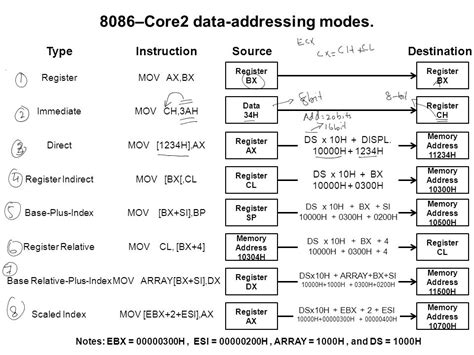
\includegraphics[width=0.7\textwidth]{../images/8086_addressing_modes.jpg}
            \caption{Mode Pengalamatan Intel 8086}
            \label{fig:8086-addressing-modes}
        \end{figure}

        \begin{table}[H]
            \centering
            \caption{Klasifikasi Mode Pengalamatan Intel 8086}
            \begin{tabular}{|p{2.8cm}|p{4.5cm}|p{7cm}|}
\hline
\textbf{Kategori} & \textbf{Mode Pengalamatan} & \textbf{Deskripsi} \\
\hline
\textbf{Register} & Register Direct & Operand berada di register \\
\hline
\textbf{Immediate} & Immediate & Operand adalah konstanta langsung \\
\hline
\textbf{Memory} & Direct, Indirect, Indexed, Based, Based-Indexed & Operand berada di memori \\
\hline
\textbf{String} & Implicit (SI, DI) & Khusus untuk operasi string \\
\hline
\textbf{I/O} & Port Direct, Port Indirect & Untuk operasi input/output \\
\hline
            \end{tabular}
            \label{tab:addressing-modes-classification}
        \end{table}

        \subsection{Mode Pengalamatan Dasar}

            \subsubsection{Pengalamatan register}
Pengalamatan register adalah mode pengalamatan yang paling efisien karena operand berada langsung di register. Mode ini tidak memerlukan akses memori tambahan dan memiliki kecepatan eksekusi tertinggi.

\textbf{Karakteristik Pengalamatan Register:}
\begin{itemize}
    \item \textbf{Kecepatan}: Paling cepat karena tidak ada akses memori
    \item \textbf{Ukuran Operand}: 8-bit atau 16-bit
    \item \textbf{Register Valid}: AX, BX, CX, DX, SI, DI, SP, BP
    \item \textbf{Kompatibilitas}: Tidak semua instruksi mendukung semua register
\end{itemize}

\begin{table}[H]
    \centering
    \caption{Contoh Pengalamatan Register}
    \begin{tabular}{|p{3.5cm}|p{3.5cm}|p{6.5cm}|}
        \hline
        \textbf{Instruksi} & \textbf{Operand} & \textbf{Keterangan} \\
        \hline
        \texttt{MOV AX, BX} & Source: BX, Destination: AX & Copy 16-bit dari BX ke AX \\
        \hline
        \texttt{ADD AL, BL} & Source: BL, Destination: AL & Add 8-bit BL ke AL \\
        \hline
        \texttt{CMP SI, DI} & Source: DI, Destination: SI & Compare SI dengan DI \\
        \hline
        \texttt{XCHG CX, DX} & Operand: CX dan DX & Exchange CX dengan DX \\
        \hline
    \end{tabular}
    \label{tab:register-addressing-examples}
\end{table}

\textbf{Keterbatasan Pengalamatan Register:}
\begin{itemize}
    \item Tidak semua instruksi mendukung semua register
    \item Beberapa instruksi memiliki register khusus (mis. MUL menggunakan AX)
    \item Register 8-bit tidak dapat digunakan untuk operasi 16-bit
\end{itemize}

            \subsubsection{Pengalamatan langsung (Immediate)}
Pengalamatan langsung menggunakan konstanta sebagai operand. Nilai konstanta disertakan langsung dalam instruksi dan tidak memerlukan akses memori untuk operand.

\textbf{Karakteristik Pengalamatan Immediate:}
\begin{itemize}
    \item \textbf{Operand}: Konstanta yang disertakan dalam instruksi
    \item \textbf{Ukuran}: 8-bit atau 16-bit
    \item \textbf{Format}: Hex (h), Decimal, Binary (b)
    \item \textbf{Posisi}: Biasanya sebagai operand kedua
\end{itemize}

\begin{table}[H]
    \centering
    \caption{Contoh Pengalamatan Immediate}
    \begin{tabular}{|p{3.5cm}|p{3.5cm}|p{6.5cm}|}
        \hline
        \textbf{Instruksi} & \textbf{Operand} & \textbf{Keterangan} \\
        \hline
        \texttt{MOV AX, 1234h} & Immediate: 1234h & Load konstanta 1234h ke AX \\
        \hline
        \texttt{ADD BX, 100} & Immediate: 100 & Add 100 ke BX \\
        \hline
        \texttt{CMP AL, 0FFh} & Immediate: 0FFh & Compare AL dengan 0FFh \\
        \hline
        \texttt{AND CX, 00FFh} & Immediate: 00FFh & AND CX dengan 00FFh \\
        \hline
    \end{tabular}
    \label{tab:immediate-addressing-examples}
\end{table}

\textbf{Format Konstanta:}
\begin{itemize}
    \item \textbf{Hexadecimal}: 1234h, 0FFh (harus diakhiri 'h')
    \item \textbf{Decimal}: 1234, 255
    \item \textbf{Binary}: 1010b (harus diakhiri 'b')
    \item \textbf{ASCII}: 'A', 'B' (untuk karakter)
\end{itemize}

            \subsubsection{Pengalamatan memori langsung}
Pengalamatan memori langsung menggunakan alamat memori yang ditentukan secara eksplisit. Alamat ini adalah offset dalam segmen default (biasanya DS).

\textbf{Karakteristik Pengalamatan Memori Langsung:}
\begin{itemize}
    \item \textbf{Operand}: Alamat memori eksplisit
    \item \textbf{Segment Default}: DS (Data Segment)
    \item \textbf{Ukuran}: 8-bit atau 16-bit
    \item \textbf{Sintaks}: [alamat] atau [offset]
\end{itemize}

\begin{table}[H]
    \centering
    \caption{Contoh Pengalamatan Memori Langsung}
    \begin{tabular}{|p{3.5cm}|p{4.0cm}|p{6.5cm}|}
        \hline
        \textbf{Instruksi} & \textbf{Operand} & \textbf{Keterangan} \\
        \hline
        \texttt{MOV AL, [1234h]} & Memory: DS:1234h & Load byte dari DS:1234h ke AL \\
        \hline
        \texttt{MOV AX, [1000h]} & Memory: DS:1000h & Load word dari DS:1000h ke AX \\
        \hline
        \texttt{MOV [2000h], BX} & Memory: DS:2000h & Store BX ke DS:2000h \\
        \hline
        \texttt{CMP [3000h], CX} & Memory: DS:3000h & Compare DS:3000h dengan CX \\
        \hline
    \end{tabular}
    \label{tab:direct-memory-addressing-examples}
\end{table}

\textbf{Segment Override:}
\begin{lstlisting}[language={[x86masm]Assembler}, caption=Segment Override dalam Pengalamatan Memori, label=lst:segment-override]
; Menggunakan segment default (DS)
mov ax, [1000h]                 ; DS:1000h

; Menggunakan segment override
mov ax, es:[1000h]              ; ES:1000h
mov ax, cs:[1000h]              ; CS:1000h
mov ax, ss:[1000h]              ; SS:1000h
\end{lstlisting}

            \subsubsection{Pengalamatan register tidak langsung}
Pengalamatan register tidak langsung menggunakan register sebagai pointer ke memori. Register berisi alamat offset yang menunjuk ke lokasi memori yang sebenarnya.

\textbf{Karakteristik Pengalamatan Register Tidak Langsung:}
\begin{itemize}
    \item \textbf{Register Valid}: BX, SI, DI, BP
    \item \textbf{Segment Default}: DS untuk BX, SI, DI; SS untuk BP
    \item \textbf{Fleksibilitas}: Register dapat diubah untuk mengakses lokasi berbeda
    \item \textbf{Efisiensi}: Lebih efisien daripada pengalamatan langsung
\end{itemize}

\begin{table}[H]
    \centering
    \caption{Contoh Pengalamatan Register Tidak Langsung}
    \begin{tabular}{|p{3.5cm}|p{3.5cm}|p{6.5cm}|}
        \hline
        \textbf{Instruksi} & \textbf{Operand} & \textbf{Keterangan} \\
        \hline
        \texttt{MOV AL, [BX]} & Memory: DS:BX & Load byte dari DS:BX ke AL \\
        \hline
        \texttt{MOV AX, [SI]} & Memory: DS:SI & Load word dari DS:SI ke AX \\
        \hline
        \texttt{MOV [DI], BX} & Memory: ES:DI & Store BX ke ES:DI \\
        \hline
        \texttt{MOV AX, [BP]} & Memory: SS:BP & Load word dari SS:BP ke AX \\
        \hline
    \end{tabular}
    \label{tab:indirect-register-addressing-examples}
\end{table}

\textbf{Contoh Penggunaan Dinamis:}
\begin{lstlisting}[language={[x86masm]Assembler}, caption=Penggunaan Dinamis Register untuk Array Access, label=lst:dynamic-usage]
; Array access dengan BX
mov bx, 0                       ; BX = index 0
mov ax, [bx]                    ; AX = array[0]

add bx, 2                       ; BX = index 1 (word array)
mov ax, [bx]                    ; AX = array[1]

; Loop dengan SI
mov si, 0                       ; SI = index awal
loop_start:
    mov ax, [si]                ; AX = array[si]
    add si, 2                   ; SI = index berikutnya
    cmp si, 20                  ; Check end condition
    jl loop_start               ; Continue loop
\end{lstlisting}

            \subsubsection{Pengalamatan berbasis indeks}
Pengalamatan berbasis indeks menggabungkan register basis/indeks dengan displacement untuk membentuk alamat memori yang fleksibel. Mode ini sangat berguna untuk akses array dan struktur data.

\textbf{Karakteristik Pengalamatan Berbasis Indeks:}
\begin{itemize}
    \item \textbf{Kombinasi Register}: BX/BP + SI/DI + displacement
    \item \textbf{Displacement}: Konstanta 8-bit atau 16-bit
    \item \textbf{Segment Default}: DS untuk BX, SI, DI; SS untuk BP
    \item \textbf{Fleksibilitas}: Sangat fleksibel untuk akses data kompleks
\end{itemize}

\begin{table}[H]
    \centering
    \caption{Kombinasi Register yang Valid untuk Pengalamatan Berbasis Indeks}
    \begin{tabular}{|p{2.8cm}|p{2.8cm}|p{7.8cm}|}
        \hline
        \textbf{Base Register} & \textbf{Index Register} & \textbf{Keterangan} \\
        \hline
        BX & SI & Kombinasi yang paling umum \\
        \hline
        BX & DI & Alternatif untuk BX+SI \\
        \hline
        BP & SI & Untuk akses stack frame \\
        \hline
        BP & DI & Alternatif untuk BP+SI \\
        \hline
    \end{tabular}
    \label{tab:indexed-addressing-combinations}
\end{table}

\begin{table}[H]
    \centering
    \caption{Contoh Pengalamatan Berbasis Indeks}
    \begin{tabular}{|p{3.5cm}|p{3.5cm}|p{6.5cm}|}
        \hline
        \textbf{Instruksi} & \textbf{Operand} & \textbf{Keterangan} \\
        \hline
        \texttt{MOV AL, [BX+SI+8]} & Memory: DS:(BX+SI+8) & Load byte dengan displacement 8 \\
        \hline
        \texttt{MOV AX, [BP+DI+16]} & Memory: SS:(BP+DI+16) & Load word dari stack frame \\
        \hline
        \texttt{MOV [BX+SI], CX} & Memory: DS:(BX+SI) & Store CX tanpa displacement \\
        \hline
        \texttt{CMP [BP+DI+4], AX} & Memory: SS:(BP+DI+4) & Compare dengan parameter stack \\
        \hline
    \end{tabular}
    \label{tab:indexed-addressing-examples}
\end{table}

\textbf{Aplikasi Praktis Pengalamatan Berbasis Indeks:}
\begin{lstlisting}[language={[x86masm]Assembler}, caption=Aplikasi Praktis Pengalamatan Berbasis Indeks, label=lst:indexed-applications]
; Akses array 2D dengan BX+SI
mov bx, 0                       ; BX = row index
mov si, 0                       ; SI = column index
mov ax, [bx+si+100h]           ; AX = array[row][col]

; Akses parameter stack dengan BP+DI
mov bp, sp                      ; BP = stack pointer
mov di, 4                       ; DI = parameter offset
mov ax, [bp+di]                 ; AX = parameter[1]

; Akses struktur data
mov bx, offset struct_data      ; BX = base address
mov si, 8                       ; SI = field offset
mov ax, [bx+si]                 ; AX = struct.field
\end{lstlisting}

            \subsubsection{Pengalamatan berbasis register}
Pengalamatan berbasis register adalah istilah umum yang mencakup berbagai variasi kombinasi register untuk pengalamatan memori. Mode ini memberikan fleksibilitas maksimal dalam akses data.

\textbf{Variasi Pengalamatan Berbasis Register:}
\begin{enumerate}
    \item \textbf{Single Register}: [BX], [SI], [DI], [BP]
    \item \textbf{Register + Displacement}: [BX+8], [SI+16], [BP+4]
    \item \textbf{Base + Index}: [BX+SI], [BP+DI]
    \item \textbf{Base + Index + Displacement}: [BX+SI+8], [BP+DI+16]
\end{enumerate}

\begin{table}[H]
    \centering
    \caption{Ringkasan Mode Pengalamatan Intel 8086}
    \begin{tabular}{|p{3.2cm}|p{3.8cm}|p{7cm}|}
        \hline
        \textbf{Mode} & \textbf{Sintaks} & \textbf{Keterangan} \\
        \hline
        \textbf{Register} & AX, BX, CX, DX & Operand di register \\
        \hline
        \textbf{Immediate} & 1234h, 100 & Konstanta langsung \\
        \hline
        \textbf{Direct Memory} & [1000h] & Alamat memori eksplisit \\
        \hline
        \textbf{Indirect} & [BX] & Register sebagai pointer \\
        \hline
        \textbf{Indexed} & [BX+SI+8] & Kombinasi register + displacement \\
        \hline
    \end{tabular}
    \label{tab:addressing-modes-summary}
\end{table}

\textbf{Contoh Program Lengkap:}
\begin{lstlisting}[language={[x86masm]Assembler}, caption=Program Lengkap dengan Berbagai Mode Pengalamatan, label=lst:complete-program]
org 100h
; Inisialisasi data segment
mov ax, data
mov ds, ax

; Pengalamatan langsung
mov ax, 1234h

; Memori langsung (absolute offset di DS)
mov al, [1234h]

; Tidak langsung via BX
mov bx, 0040h
mov al, [bx]

; Berbasis indeks
mov si, 0010h
mov dl, [bx+si+5]

int 20h

segment data
msg db 'Hello World!', 0
\end{lstlisting}

    \section{Struktur File Assembly}

        \subsection{Format Dasar Program Assembly}
            Program assembly Intel 8086 dapat dikompilasi menjadi dua format utama: \texttt{.COM} dan \texttt{.EXE}.

            \begin{table}[H]
\centering
\caption{Perbandingan Format Program Assembly}
\begin{tabular}{|p{1.8cm}|p{6.0cm}|p{6.5cm}|}
    \hline
    \textbf{Format} & \textbf{Karakteristik} & \textbf{Penggunaan} \\
    \hline
    \texttt{.COM} & \begin{itemize}
    \item Ukuran maksimal 64 KB
    \item Segmen tunggal (code=data=stack)
    \item \texttt{org 100h} untuk PSP
    \item Entry point di offset 100h
    \end{itemize} & Program kecil dan sederhana \\
    \hline
    \texttt{.EXE} & \begin{itemize}
    \item Ukuran tidak terbatas
    \item Multiple segments
    \item Entry point fleksibel
    \item Mendukung relokasi
    \end{itemize} & Program kompleks dan besar \\
    \hline
\end{tabular}
\label{tab:assembly-program-formats}
            \end{table}

        \subsection{Direktif Assembler Penting}
            Direktif assembler memberikan instruksi kepada assembler tentang bagaimana mengatur kode dan data.

            \begin{table}[H]
\centering
\caption{Direktif Assembler Umum}
\begin{tabular}{|p{2.8cm}|p{4.2cm}|p{7cm}|}
    \hline
    \textbf{Direktif} & \textbf{Fungsi} & \textbf{Contoh Penggunaan} \\
    \hline
    \texttt{ORG} & Menentukan origin address & \texttt{org 100h} (COM) atau \texttt{org 0} (EXE) \\
    \hline
    \texttt{DB/DW/DD} & Define byte/word/dword & \texttt{msg db 'Hello', 0} \\
    \hline
    \texttt{SEGMENT/ENDS} & Mendefinisikan segmen & \texttt{code segment ... code ends} \\
    \hline
    \texttt{ASSUME} & Menentukan segment register & \texttt{assume cs:code, ds:data} \\
    \hline
    \texttt{END} & Akhir program & \texttt{end start} atau \texttt{end} \\
    \hline
\end{tabular}
\label{tab:assembly-directives}
            \end{table}

        \subsection{Organisasi Program yang Baik}
            \begin{itemize}
\item \textbf{Pemisahan Segmen}: Pisahkan kode, data, dan stack dalam segmen terpisah
\item \textbf{Label Deskriptif}: Gunakan nama yang menjelaskan fungsi (mis. \texttt{calculate\_sum})
\item \textbf{Komentar Jelas}: Jelaskan tujuan, bukan instruksi yang sudah jelas
\item \textbf{Konvensi Penamaan}: Konsisten dalam penamaan variabel dan prosedur
\item \textbf{Dokumentasi Register}: Catat register yang digunakan/dimodifikasi oleh setiap prosedur
            \end{itemize}


\end{document}
